%%
%% 1. Vorlesung <2012-10-16 Tue>
%% 
%% Skript Differentialgeometrie im Wintersemester 12/13
%% Zur Vorlesung von Dr. Grensing am KIT Karlsruhe
%%
%% Mitschrieb und Textsatz von Jan-Bernhard Kordaß.
%%

\section*{"Ubersicht}

\begin{itemize}
\item Mannigfaltigkeiten, Tangentialvektoren
\item Kovariante Ableitung
\item Riemannsche Metriken
\item Krümmung
\item Jacobifelder
\item Satz von Bonnet
\end{itemize}

\chapter{Differenzierbare Mannigfaltigkeiten}

\begin{dfn}
  Eine $n$-dimensionale \CmMark[Mannigfaltigkeit!topologische]{topologische Mannigfaltigkeit} $M$ ist ein topologischer \gls{Hausdorff-Raum} mit einer abzählbaren Basis der \gls{Topologie} in dem zu jedem Punkt $p \in M$ eine offene Menge $U$ mit $p \in U$ existiert und ein \gls{Homoeomorphismus} $\phi \colon U \to V$ auf eine offene Menge $V \subset \R^{n}$.

% Abbildung 1-1
%\CmPutSvg{1-1-topologische-mf}{8.5cm}
\begin{center}\begin{tikzpicture}[font=\scriptsize]
	\draw[->] (-1.5,0) to[out=20, in=160]node[above,font=\scriptsize]{$\phi' \circ \phi^{-1}$} (1.5,0);
	
	\draw[->] (-4,-0.5) -- (-2,-0.5); \draw[->] (-3.75,-0.75) -- (-3.75, 1.25); \node[font=\scriptsize] at (-4, 1.25) {$\R^n$};
	\draw[->] (2,-0.5) -- (4,-0.5); \draw[->] (2.25,-0.75) -- (2.25, 1.25); \node[font=\scriptsize] at (2, 1.25) {$\R^m$};
	
	\node[font=\scriptsize] at (0,2) {$U \cap U' \ne 0$};
	
	\draw (-4.25, 1.75) to[out=70,in=180] (-1.75,3) to[out=300,in=90] (-1.25, 1.25) to[out=180,in=340] (-4.25, 1.75) -- cycle; \node at (-1.25,3) {$M$};
	\filldraw[fill=gray!20] (-2.75,2) circle(0.4); \node[font=\scriptsize] at (-3.25,2.25) {$U$};
	\filldraw[fill=gray!20] (-3,0.25) circle (0.5); \node at (-2.25, 0.5) {$V$};
	\draw[->] (-2.75,1.5) to[out=280,in=80] node[right]{$\phi$} (-2.75,0.75);
			
	\draw (1.75, 1.75) to[out=70,in=180] (4.25,3) to[out=300,in=90] (4.75, 1.25) to[out=180,in=340] (1.75, 1.75) -- cycle; \node at (4.75,3) {$M$};
	\filldraw[fill=gray!20] (3.55,2.25) circle(0.6); \node[font=\scriptsize] at (2.75,2.25) {$U'$};
		
	\coordinate (ctrl0up) at ($(2.5,-0.25) + 0.2*(0.5,2)$); \coordinate (ctrl0down) at ($(2.5,-0.25) + 0.2*(0,-1.5)$);
	\coordinate (ctrl1down) at ($(3,0.25) - 0.1*(0.5,1)$); \coordinate (ctrl1up) at ($(3,0.25) + 0.1*(0.5,1)$);
	\coordinate (ctrl2down) at ($(3,0.7) - 0.1*(0.5,1)$); \coordinate (ctrl2up) at ($(3,0.7) + 0.1*(0.5,1)$);
	\coordinate (ctrl3down) at ($(4,0.5) + 0.3*(-0.5,1)$); \coordinate (ctrl3up) at ($(4,0.5) - 0.3*(-0.25,1)$);
	\coordinate (ctrl4down) at ($(3.75,-0.3) + 0.2*(0.8,1)$); \coordinate (ctrl4up) at ($(3.75,-0.3) - 0.2*(0.7,0.75)$);
	\begin{scope}
		\fill[gray!20] (2.5,-0.25) ..controls(ctrl0up) and (ctrl1down).. (3,0.25) ..controls(ctrl1up) and (ctrl2down).. (3,0.7) ..controls(ctrl2up) and (ctrl3down).. (4,0.5) ..controls(ctrl3up) and (ctrl4down).. (3.75,-0.3) ..controls(ctrl4up) and (ctrl0down).. (2.5,-0.25); \node at (4.25, 0.5) {$V'$};
		\clip(2.5,-0.25) ..controls(ctrl0up) and (ctrl1down).. (3,0.25) ..controls(ctrl1up) and (ctrl2down).. (3,0.7) ..controls(ctrl2up) and (ctrl3down).. (4,0.5) ..controls(ctrl3up) and (ctrl4down).. (3.75,-0.3) ..controls(ctrl4up) and (ctrl0down).. (2.5,-0.25); \node at (4.25, 0.5) {$V'$};
		\fill[gray] (2,0) circle (1);
		 (2.5,-0.25) ..controls(ctrl0up) and (ctrl1down).. (3,0.25) ..controls(ctrl1up) and (ctrl2down).. (3,0.7) ..controls(ctrl2up) and (ctrl3down).. (4,0.5) ..controls(ctrl3up) and (ctrl4down).. (3.75,-0.3) ..controls(ctrl4up) and (ctrl0down).. (2.5,-0.25); \node at (4.25, 0.5) {$V'$};
	\end{scope}
	\draw  (2.5,-0.25) ..controls(ctrl0up) and (ctrl1down).. (3,0.25) ..controls(ctrl1up) and (ctrl2down).. (3,0.7) ..controls(ctrl2up) and (ctrl3down).. (4,0.5) ..controls(ctrl3up) and (ctrl4down).. (3.75,-0.3) ..controls(ctrl4up) and (ctrl0down).. (2.5,-0.25) -- cycle; \node at (4.25, 0.5) {$V'$};
	\draw[->] (3.5,1.5) to[out=280,in=80] node[right]{$\phi'$} (3.5,0.75);
\end{tikzpicture}\end{center}

  $\phi' \circ \phi^{-1}$ ist ein Hom"oomorphismus offener Mengen des $\R^n$ bzw. $\R^m$. Nach dem \href{http://de.wikipedia.org/wiki/Fixpunktsatz_von_Brouwer}{Satz von Brouwer} (1912) gilt dann $m = n$. Damit ist die Dimension einer zusammenh"angenden topologischen Mannigfaltigkeit eindeutig definiert.\\

  Die Abbildung $\phi \colon U \to V \subset \R^n$ hei\ss t \CmMark{Karte} von $M$ um $p$, die Menge $U$ hei\ss t \CmMark{Kartengebiet}.\\

  Eine Menge von Karten $\mathcal A = \{(\phi_{\alpha}, U_{\alpha}) \mid \alpha \in J \}$ hei\ss t \CmMark{Atlas} von $M$, falls $\bigcup_{\alpha \in J}U_{\alpha} = M$.\\

  Ein Atlas $\mathcal A$ von $M$ hei\ss t $C^k$-Atlas, wenn für alle $\alpha, \beta \in J$ mit $U_{\alpha} \cap U_{\beta} \neq \emptyset$ der sogenannte \CmMark{Kartenwechsel}:
  \begin{align*}
    \phi_{\beta} \circ \phi_{\alpha}^{-1}\colon \phi_{\alpha}(U_{\alpha} \cap U_{\beta}) \to \phi_{\beta}(U_{\alpha} \cap U_{\beta})
  \end{align*}
  ein $C^k$-\gls{Diffeomorphismus} ist.

  \begin{center}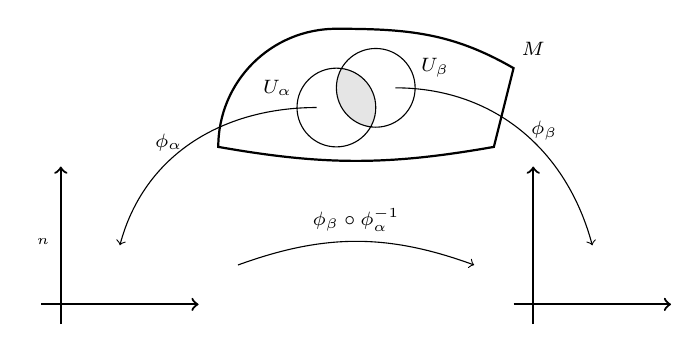
\begin{tikzpicture}[font=\scriptsize]
  	\draw[->] (-1.5,0) to[out=20, in=160]node[above,font=\scriptsize]{$\phi_\beta \circ \phi^{-1}_\alpha$} (1.5,0);
	
	\draw[->,thick] (-4,-0.5) -- (-2,-0.5); \draw[->,thick] (-3.75,-0.75) --node[left]{$\R^n$} (-3.75, 1.25);
	\draw[->,thick] (2,-0.5) -- (4,-0.5); \draw[->,thick] (2.25,-0.75) -- (2.25, 1.25);
	
	\draw[thick]  (-0.25, 3) to[out=0,in = 150] (2,2.5) -- (1.75, 1.5) to[out=190,in=350] (-1.75, 1.5) to[out=90,in=180] (-0.25, 3) -- cycle; \node at (2.25,2.75) {$M$};
	
	\begin{scope}
		\clip (0.25,2.25) circle(0.5);
		\clip (-0.25,2) circle(0.5);
		\fill[gray!20] (0,2) circle(1);
	\end{scope}
	\draw (0.25,2.25) circle(0.5) (-0.25,2) circle(0.5); \node at (-1, 2.25) {$U_\alpha$}; \node at (1,2.5) {$U_\beta$};
	
	\draw[->] (-0.5,2) to[out=180,in=75] node[left]{$\phi_\alpha$} (-3,0.25);
	\draw[->] (0.5,2.25) to[out=0,in=105] node[right]{$\phi_\beta$} (3,0.25);
  \end{tikzpicture}\end{center}


  Eine Karte $\psi \colon U \to V$ von $M$ hei\ss t \CmMark[Karte!vertr{\"a}gliche]{verträglich} mit einem $C^k$-Atlas $\mathcal A = \{(\phi_{\alpha},U_{\alpha}) \mid \alpha \in J\}$ wenn jeder Kartenwechsel
  \begin{align*}
    \phi_{\alpha} \circ \psi^{-1}: \psi(U \cap U_{\alpha}) \to \phi_{\alpha}(U \cap U_{\alpha})
  \end{align*}
  ein $C^k$-Diffeomorphismus ist, also $\mathcal A' = \mathcal A \cup \{(\psi, U)\}$ ebenfalls ein $C^k$-Atlas ist. Die Menge aller mit $\mathcal A$ verträglichen Karten ist ein \CmMark[Atlas!maximaler]{maximaler $C^k$-Atlas}. Jeder maximale Atlas enthält alle mit ihm verträglichen Karten. Ein maximaler $C^k$-Atlas hei\ss t auch \CmMark{$C^k$-differenzierbare Struktur}.

\end{dfn}

\begin{Dfn}[differenzierbare Mannigfaltigkeit]
  Eine \CmMark[Mannigfaltigkeit!differenzierbare]{differenzierbare Mannigfaltigkeit} der Klasse $C^k$ ist eine topologische Mannigfaltigkeit zusammen mit einer $C^{k}$-differenzierbaren Struktur.\\
\end{Dfn}

\begin{bsp}
  Einige Beispiele f"ur glatte Mannigfaltigkeiten:
  \begin{enumerate}[leftmargin=*,label=\arabic*)]
  \item $M = \R^n, \mathcal A = \{(\Id_{\R^n},\R^n)\}$
  \item $M \subset \R^n$ offen, $\mathcal A = \{(\imath_{M},M)\}$
  \item $S^1 \subset \R^2$ ist eine eindimensionale $C^{\infty}$-Mannigfaltigkeit:
    \begin{align*}
      U = \{(\sin t, \cos t) \mid t \in (0,2\pi)\}
    \end{align*}

    % Abbildung 1-3
    \marginnote{\begin{center}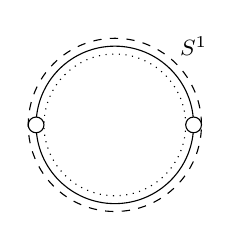
\begin{tikzpicture}[font=\footnotesize]
    		%\draw[step=0.25,gray!15] (-1,-1) grid (1,1); \draw[step=0.5,gray!30] (-1,-1) grid (1,1); \fill (0,0) circle(0.1); %Hilfsgitter
		\draw (0,0) circle (1); \draw[dashed] (0,0) circle (1.1); \draw[dotted] (0,0) circle (0.9); \node at (1,1) {$S^1$};
		\filldraw[fill=white] (-1,0) circle (0.1) (1,0) circle (0.1);
    \end{tikzpicture}\\
    \textcolor{gray}{$S^1$ Einheitskreis}
    \end{center}}[-2cm]
    % \CmMarginSvg[-2cm]{1-3-karten-der-s1}{3cm}

    ist offen in $S^1$ und die Kartenabbildung
    \begin{align*}
      \phi \colon (\sin t, \cos t) \mapsto t
    \end{align*}
    ist ein Hom"oomorphismus.
    \begin{align*}
      \phi' \colon U' = \{(\sin t, \cos t) \mid t \in (-\pi,\pi)\} \to (-\pi,\pi)
    \end{align*}
    ebenfalls. $\mathcal A = \{(\phi, U), (\phi',U')\}$ ist ein Atlas von $S^1$, denn $U \cup U' = S^1$.
    \begin{align*}
      & \phi' \circ \phi^{-1} \colon \phi(U \cap U') \to \phi'(U \cap U')\\
      & (0,\pi)\cup(\pi,2\pi) \to (-\pi,0)\cup(0,\pi), t \mapsto \begin{cases}
        t & 0 < t < \pi\\
        t-2\pi & \pi < t < 2\pi
      \end{cases}
    \end{align*}

  \item Jeder reelle Vektorraum endlicher Dimension ist in kanonischer Weise eine $C^{\infty}$-Mannigfaltigkeit.\\
    W"ahle eine Basis $\{v_1, \ldots, v_n\}$ von $V$. Diese definiert mit
    \begin{align*}
      \phi\left(\sum\lambda_iv_i\right) = (\lambda_1, \ldots, \lambda_n)
    \end{align*}
    eine Bijektion auf $\R^n$. Damit erhält man eine globale Karte von $V$.
    Der zugehörige Atlas h"angt nicht von der Wahl der Basis ab, denn ist $\{w_1, \ldots, w_n\}$ eine weitere Basis von $V$ und $\psi(\sum \lambda_iw_i) = (\lambda_1, \ldots, \lambda_n)$ eine weitere Karte, so ist $\phi \circ \psi^{-1}$ als \gls{Endomorphismus} des $\R^n$ schon $C^{\infty}$.

  \item $S^n = \{(x^0, x^1, \ldots, x^n) \mid \sum_{i = 0}^n(x^{i})^2 = 1\}$.\\

    % Abbildung 1.4
    %\CmMarginSvg{1-4-s3-sphaere}{3.5cm}
    \marginnote{\begin{center}\begin{tikzpicture}[font=\scriptsize]
    		%\draw[step=0.25,gray!15] (-1,-1) grid (1,1); \draw[step=0.5,gray!30] (-1,-1) grid (1,1); \fill (0,0) circle(0.1); %Hilfsgitter
		% Koordinatenachsen mit Beschriftung
		\draw[->] (0,-1.25) -- (0,1.5) node[left]{$x^0$}; \draw[->] (-1.25,0) -- (1.5,0) node[below]{$x^1$}; \draw[->] (1,1) -- (-1.25,-1.25) node[right]{$x^2$}; \node at (1.25, 1.5) {$S^2 \subset \R^3$};
		% Kreis, Ellipse und Gerade (verwende Namen um Schnittpunkt bestimmen zu koennen)
		\path[draw, thick, name path=kreis] (0,0) circle (1) ellipse(1 and 0.45); \path[draw,name path=gerade] (0,1) -- (1,-1.25);
		% Punkte N und p
		\filldraw[fill=white] (0,1) circle (0.05) node[anchor=south west,xshift=-2,yshift=-1.5]{$N$} ($(0,1)+0.35*(1,-1.25)-0.35*(0,1)$) circle (0.05) node[right]{$p$};
		% Punkt phi(p) bei Schnittpunkt von Gerade und Kreis
		\path [name intersections={of=kreis and gerade}]; \filldraw[fill=white] (intersection-2) circle(0.05) node[right]{$\phi(p)$};
	\end{tikzpicture}\end{center}}%[3.5cm]
    
    Betrachte den Nordpol $N = (1,0,\ldots,0)$ und den S"udpol $S = (-1,0,\ldots,0)$ und die Abbildung
    \begin{align*}
      & \phi \colon U = S^{n}\setminus\{N\} \to \R^n, x \mapsto \left(\frac{x^1}{1-x^0}, \ldots, \frac{x^{n}}{1-x^0}\right),\\
      & \psi \colon U' = S^{n} \setminus \{S\} \to \R^n, x \mapsto \left(\frac{x^1}{1+x^0}, \ldots, \frac{x^n}{1+x^0}\right)
    \end{align*}

    Aufgabe: Zeige, dass $(\phi, U), (\psi, U')$ einen $C^{\infty}$-Atlas auf $S^n$ definiert.

  \end{enumerate}
\end{bsp}

\begin{Dfn}[Differenzierbare Abbildungen]
Eine stetige Abbildung $f \colon M \to N$ zwischen glatten Mannigfaltigkeiten $M$ und $N$ hei\ss t \CmMark{glatt} ($C^{\infty}$-differenzierbar), wenn es zu jedem $p \in M$ Karten $(\phi, U)$ in $M$ um $p$ und geeignete $(\phi', U')$ in $N$ um $f(p)$ gibt, so dass $\phi' \circ f\circ\phi^{-1}$ glatt ist.
% Abbildung 1-5
%\CmPutSvg{1-5-glatte-abb}{9cm}
\begin{center}\begin{tikzpicture}[font=\scriptsize]
	%\draw[step=0.25,gray!15] (-5,-1) grid (5,5); \draw[step=0.5,gray!30] (-5,-1) grid (5,5); \fill (0,0) circle(0.1); %Hilfsgitter
	
	% Die Abbildungspfeile
	\draw[->] (-1.5,0) to[out=20, in=160]node[above]{$\phi' \circ f \circ \phi^{-1}$} (1.5,0);
	\draw[->] (-1,2) --node[above]{$f$} (1.5,2);
	
	% Die Achsen
	\draw[->,thick] (-4.5,-0.5) -- (-2,-0.5); \draw[->,thick] (-4.25,-0.75) --node[left]{$\R^n$} (-4.25, 1.25);
	\draw[->,thick] (2,-0.5) -- (4.5,-0.5); \draw[->,thick] (2.25,-0.75) --node[left]{$\R^m$} (2.25, 1.25);
	
	% Die Blasen
	\draw[thick] (-4.25, 1.75) to[out=70,in=180] (-1.75,3) to[out=300,in=90] (-1.25, 1.25) to[out=180,in=340] (-4.25, 1.75) -- cycle; \node[font=\normalfont] at (-1.25,3) {$M$};
	\draw[thick] (1.75, 1.75) to[out=70,in=180] (4.25,3) to[out=300,in=90] (4.75, 1.25) to[out=180,in=340] (1.75, 1.75) -- cycle; \node[font=\normalfont] at (4.75,3) {$N$};
	
	% Die linke Kartoffel (zuerst werden die Punkte definiert, dann die Richtungsvektoren der Splines, dann die Kartoffel selbst)
	\coordinate (kartoffel0l) at (-3.25,1.75); \coordinate (kartoffel1l) at (-3.25,2.5); \coordinate (kartoffel2l) at (-2.25,2.25); \coordinate (kartoffel3l) at (-2.5,1.75);
	\coordinate (ctrlk0l) at (-0.25,0.5); \coordinate (ctrlk1l) at (0.5,0.25); \coordinate (ctrlk2l) at (-0.25,1); \coordinate (ctrlk3l) at (2,0.25);
	\draw (kartoffel0l) ..controls($(kartoffel0l)+0.5*(ctrlk0l)$) and ($(kartoffel1l)-0.3*(ctrlk1l)$).. (kartoffel1l) ..controls($(kartoffel1l)+0.6*(ctrlk1l)$) and($(kartoffel2l)+0.45*(ctrlk2l)$).. (kartoffel2l) ..controls($(kartoffel2l)-0.25*(ctrlk2l)$) and ($(kartoffel3l)+0.15*(ctrlk3l)$).. (kartoffel3l)  ..controls($(kartoffel3l)-0.1*(ctrlk3l)$) and ($(kartoffel0l)-0.9*(ctrlk0l)$).. (kartoffel0l); \node at (-3.5,2.25) {$U$};
	% Der Punkt in der Kartoffel, der Pfeils raus und der Kreis
	\draw[->] (-2.75,2) node[right]{$p$} to[out=280,in=80] node[right]{$\phi$} (-2.75,0); \fill (-2.75,2) circle (0.05);
	\draw (-3,0.25) circle(0.5); \node at (-3.5,0.75) {$V$};
	
	% Die rechte Kartoffel
	\coordinate (kartoffel0r) at (3.25,1.75); \coordinate (kartoffel1r) at (3.5,2.5); \coordinate (kartoffel2r) at (4.5,2.25); \coordinate (kartoffel3r) at (4.25,1.5);
	\coordinate (ctrlk0r) at (-0.25,0.5); \coordinate (ctrlk1r) at (-0.25,0.25); \coordinate (ctrlk2r) at (-0.25,0.5); \coordinate (ctrlk3r) at (0.25,0);
	\draw (kartoffel0r) ..controls($(kartoffel0r)+0.5*(ctrlk0r)$) and ($(kartoffel1r)-(ctrlk1r)$).. (kartoffel1r) ..controls($(kartoffel1r)+(ctrlk1r)$) and ($(kartoffel2r)+(ctrlk2r)$).. (kartoffel2r) ..controls($(kartoffel2r)-(ctrlk2r)$) and ($(kartoffel3r)+(ctrlk3r)$).. (kartoffel3r) ..controls($(kartoffel3r)-(ctrlk3r)$) and ($(kartoffel0r)-(ctrlk0r)$).. (kartoffel0r); \node at (3.25,2.25) {$U'$};
	
	\draw[->] (3.75,2) node[right]{$f(p)$} to[out=280,in=80] node[right]{$\phi'$} (3.75,0); \fill (3.75,2) circle (0.05);
	\draw (3.5,0.25) circle(0.5); \node at (3,0.75) {$V'$};
\end{tikzpicture}

% Korrektur
% \textcolor{red}{Sollte das in der Zeichnung beim unteren Pfeil nicht $\phi'\circ f \circ \phi^{-1}$ hei\ss en?}
% Ja! sollte es! (JB, <2012-11-9 Fri>)

\end{center}

Die Menge aller glatten Abbildungen von $M$ nach $N$ wird $C^{\infty}(M,N)$ genannt.
\end{Dfn}

\begin{emptythm}[Konvention:]
Ab jetzt seien zunächst alle Mannigfaltigkeiten, wie auch alle Abbildungen als glatt vorrausgesetzt.
\end{emptythm}

\begin{bem}
  Da Kartenwechsel $C^{\infty}$ sind, gilt obige Bedingung automatisch für alle Karten von $M$ und $N$ (evtl. nach Einschränkung).
\end{bem}

\begin{bsp}
  Es folgen zwei Beispiele für differenzierbare Abbildungen:
  \begin{enumerate}
  \item $(\phi,U) \in \mathcal A \Rightarrow \phi \in C^{\infty}(U,\R^n)$, denn
    \begin{align*}
      \Id_{\R^n}\circ \phi \circ \phi^{-1} = \phi \circ \phi^{-1} \in C^{\infty}.
    \end{align*}
  \item $f \in C^{\infty}(M,N), \ g \in C^{\infty}(N,P) \Rightarrow g \circ f \in C^{\infty}(M,P)$, denn
    \begin{align*}
      \phi_p \circ g \circ f \circ \phi^{-1}_m = (\phi_p \circ g \circ \phi_n^{-1}) \circ (\phi_n \circ f \circ \phi_m^{-1}) \in C^{\infty}.
    \end{align*}
  \end{enumerate}
\end{bsp}

\begin{Dfn}[Diffeomorphismus]
Eine Abbildung $f \colon M \to N$ hei\ss t \CmMark{Diffeomorphismus}, wenn $f$ bijektiv ist und $f$, sowie $f^{-1}$ $C^{\infty}$-Abbildungen von $M$ nach $N$ sind. Insbesondere haben $M$ und $N$ in diesem Fall dieselbe Dimension. Die Menge der Diffeomorphismen von $M$ nach $M$ wird mit $\Diff(M)$ bezeichnet. $(\Diff(M), \circ)$ ist bez"uglich der Hintereinanderausf"uhrung eine Gruppe.
\end{Dfn}


% 2. Vorlesung <2012-10-19 Fri>

\section{Produkte von Mannigfaltigkeiten}

Es seien $M$ und $N$ glatte Mannigfaltigkeiten der Dimensionen $m$ und $n$. Dann hat $M \times N$ versehen mit der \gls{Produkttopologie}, die Struktur einer Mannigfaltigkeit. Da $M$ und $N$ hausdorffsch sind und abzählbare Basen ihrer Topologie besitzen gilt dies auch für $M \times N$.
Sind $(\phi, U)$ und $(\psi, V)$ Karten von $M$ bzw. $N$, so ist $\phi \times \psi$ ein Homöomorphismus von $U \times V$ auf sein offenes Bild in $\R^m \times \R^n \cong \R^{m + n}$.

Seien $\mathcal A = \{(\phi_{\alpha}, U_{\alpha}) \mid \alpha \in \calI \}$ und $\mathcal A' = \{(\psi_{\beta}, V_{\beta}) \mid \beta \in \calJ\}$ $C^{\infty}$-Atlanten von $M$ und $N$. Dann ist $\mathcal B = \{(\phi_{\alpha}\times\psi_{\beta},U_{\alpha}\times V_{\beta}) \mid (\alpha, \beta) \in \calI \times \calJ\}$ ein $C^{\infty}$-Atlas von $M\times N$, denn 
\begin{align*}
  (\phi_{\alpha} \times \psi_{\beta}) \circ (\phi_{\mu} \times \psi_{\nu})^{-1} = (\phi_{\alpha} \circ \phi_{\mu}^{-1}) \times (\psi_{\beta} \circ \psi_{\nu}^{-1})
\end{align*}
ist ein $C^{\infty}$-Diffeomorphismus. Damit ist $M\times N$ in kanonischer Weise eine glatte $(m+n)$-dimensionale Mannigfaltigkeit. Die kanonischen Projektionen $\pi_M\colon M\times N \to M, \ \pi_N\colon M \times N \to N$ und die Abbildung $\tau \colon M \times N \to N \times M, (p,q) \mapsto (q,p)$ sind glatte Abbildungen.

\begin{bsp}\marginnote{\begin{tikzpicture}[scale=0.9,font=\scriptsize]
	%\draw[step=0.25,gray!15] (0,-2) grid (3,2); \draw[step=0.5,gray!30] (0,-2) grid (3,2); \fill (0,0) circle(0.1); %Hilfsgitter
	\tikztorus{(0,0)};
	\draw (0,0) ellipse (1.5 and 0.7*\torushoehe);
	\begin{scope}
		\clip (torusUntenLoch) rectangle ($(torusUnten)-(0.25,0)$);
		\draw ($0.5*(torusUntenLoch) + 0.5*(torusUnten)$) ellipse (0.2 and 0.5*\torusdicke);
	\end{scope}\begin{scope}
		\clip (torusUntenLoch) rectangle ($(torusUnten)+(0.25,0)$);
		\draw[dashed] ($0.5*(torusUntenLoch) + 0.5*(torusUnten)$) ellipse (0.2 and 0.5*\torusdicke);
	\end{scope}
	\node[below,font=\scriptsize] at (torusUnten) {$S^1$}; \node[font=\normalsize] at (-1.5,1) {$T^2$};
	\draw[->] (1.75,1) node[right]{$S^1$} to[out=180,in=450] (1.25,0.5);
\end{tikzpicture}}
Es folgen einige Beispiele für Produkt-Mannigfaltigkeiten:
\begin{enumerate}[label=\arabic*)]
\item
	Zylinder $\R \times S^1$
\item
	$T^n = \bigtimes_{i=1}^nS^1$
  
    $\iota: \R^m \hookrightarrow \R^n$, $(x^1,\ldots ,x^m) \mapsto (x^1,\ldots ,x^m,0, 0,\ldots)$
\end{enumerate}
\end{bsp}


\section{Untermannigfaltigkeiten}

\begin{Dfn}[Untermannigfaltigkeit]\label{def-1-4}
  Es sei $N$ eine glatte Mannigfaltigkeit. Eine Teilmenge $M \subseteq N$ heißt \CmMark{Untermannigfaltigkeit} von $N$, wenn für alle $p \in M$ eine Karte $(\phi, U)$ von $N$ um $p$ existiert, so dass
  \begin{align*}
    \phi(U \cap M) = \phi(U) \cap \underbrace{(\R^m \times \{0\})}_{\mathclap{\{(x^1,\ldots,x^m,0,\ldots,0) \in \R^m\times\R^{n-m} \cong \R^{n} \}}}
  \end{align*}
gilt. Eine solche Karte heißt an $M$ \CmMark[Karte!adaptierte]{adaptierte Karte}. Die Zahl $n-m$ heißt \CmMark{Kodimension} von $M$ in $N$.

% Abbildung 1-7
%\CmPutSvg{1-7-untermf}{8cm}
\begin{center}\begin{tikzpicture}[font=\scriptsize,scale=0.9]
	%\draw[step=0.25,gray!15] (-6,-1) grid (6,5); \draw[step=0.5,gray!30] (-6,-1) grid (6,5); \fill (0,0) circle(0.1); %Hilfsgitter
	
	\draw[->] (1.5,-0.5) -- (5.5,-0.5)node[below]{$\R^m$}; \draw[->] (1.5,-0.5) -- (1.5,2.5)node[left]{$\R^{n-m}$}; \draw[ultra thick] (1.5,-0.5) --node[above]{$\phi(U\cap M)$} (4,-0.5); \node at (4.5,2) {$\R^n$};
	
	\draw[->] (-3,0.75) to[out=330,in=180]node[below]{$\phi$} (1,0);
	
	\coordinate(1) at (-0.25,2.75); \coordinate(2) at (-5.25,1.25); \coordinate(3) at (-4.25,4.25);
	\coordinate(ctrl1) at (0,-1.25); \coordinate(ctrl2) at (1.75,-1); \coordinate(ctrl3) at (-0.5,-0.25);
	\draw (1) ..controls($(1)+(ctrl1)$) and($(2)+(ctrl2)$).. (2) ..controls($(2)-(ctrl2)$) and($(3)+(ctrl3)$).. (3);
	
	\coordinate (a) at (-1.25, 2.75); \coordinate (b) at (-3.5, 1.75); \coordinate (c) at (-4.25, 1.75); \coordinate (d) at (-4.5, 2.25); \coordinate (e) at (-5, 2.5); \coordinate (f) at (-4.25, 3.5);
	\coordinate (ctrlb) at (1,0); \coordinate (ctrlc) at (0.52,-0.25); \coordinate (ctrle) at (0,-0.25);
	\draw[very thick] (a) ..controls(a) and ($(b) + 1.75*(ctrlb)$).. (b) ..controls($(b) - 0.5*(ctrlb)$) and ($(c) + 0.5*(ctrlc)$).. (c) ..controls($(c) - 0.5*(ctrlc)$) and ($(d) + 0.5*(ctrlc)$).. (d) ..controls($(d) - 0.5*(ctrlc)$) and ($(e) + 0.5*(ctrle)$).. (e) ..controls($(e) - 2*(ctrle)$) and(f).. (f);
	
	\filldraw[fill=white] (b) circle(0.05) node[anchor=north west]{$p$}; \draw (b) circle(0.5); \node at (-4,1.25) {$U$}; \node at (-1.75,2) {$M$}; \node at (-5.5,3.5) {$N$};
	
	\coordinate (cntr) at (-3,3);
	\begin{scope}
		\clip ($(cntr)-(1,0.6)$) rectangle ($(cntr)+(1,-0.1)$);
		\draw[name path=l] (cntr) ellipse(1 and 0.5);
	\end{scope}
	\path[name path=u] ($(cntr) - (0,0.5)$) ellipse(0.75 and 0.5);
	\path[name intersections={of=u and l}];
	\begin{scope}
		\clip (intersection-1) rectangle ($(intersection-2)+(0,0.5)$);
		\draw ($(cntr) - (0,0.5)$) ellipse(0.75 and 0.5);
	\end{scope}
\end{tikzpicture}\end{center}

\end{Dfn}

\begin{Lemma}\label{lemma-1-5}
  Es seien $N$ eine $n$-dimensionale glatte Mannigfaltigkeit und $M \subseteq N$ eine $m$-dimensionale Untermannigfaltigkeit von $N$. Bezeichnet $\mathcal A$ einen $C^{\infty}$-Atlas von $N$ und $\pi \colon \R^n \to \R^m, (x^1, \ldots, x^m,\ldots,x^n) \mapsto (x^1, \ldots, x^m)$, so ist
  \begin{align*}
    \mathcal B = \{(\pi \circ \phi|_{U \cap M},U\cap M) \mid (\phi, U) \in \mathcal A \text{ an } M \text{ adaptierte Karte}\}
  \end{align*}
  ein $C^{\infty}$-Atlas von $M$.
\end{Lemma}

\begin{bew}
  Die Hausdorff-Eigenschaft und die Abzählbarkeit der Topologie werden von $N$ auf $M$ vererbt.\\
  Ist $p \in N$, so existiert eine adaptierte Karte $(\phi,U)$ von $N$ um $p$ und $\pi \circ \phi|_{U \cap M}$ ist ein Homöomorphismus von $U \cap M$ auf eine offene Teilmenge des $\R^m$. Jeder Kartenwechsel
  \begin{align*}
    (\pi \circ \phi|_{U \cap M}) \circ (\pi \circ \psi|_{V \cap M})^{-1} = (\pi \circ \phi) \circ (\psi^{-1} \circ \imath) = \pi \circ (\phi \circ \psi^{-1}) \circ \imath
  \end{align*}
  ist ein $C^{\infty}$-Diffeomorphismus.
\end{bew}

\begin{bem}
  Erinnerung: $M \subseteq \R^n$ heißt glatte $n$-dimensionale Untermannigfaltigkeit des $\R^n$, wenn für alle $p \in M$ eine offene Umgebung $U$ und eine Abbildung $\phi \colon U \to \R^n$  mit folgenden Eigenschaften existiert:
  \begin{enumerate}[label=(\roman*),widest=ii]
  \item $\phi \colon U \to \phi(U)$ ist ein Diffeomorphismus auf sein offenes Bild im $\R^{n}$.
  \item $\phi(U \cap M) = \phi(U) \cap (\R^{m} \times \{0\})$.
  \end{enumerate}
Jedes solche $M$ ist eine Untermannigfaltigkeit im Sinne von Definition \ref{def-1-4}, denn jedes $\phi$ wie oben ist wegen (i) eine Karte von $\R^n$ (im Sinne glatter Mannigfaltigkeiten) und wegen (ii) eine an $M$ adaptierte Karte. Also sind mit Lemma \ref{lemma-1-5} glatte Untermannigfaltigkeiten des $\R^n$ glatte Mannigfaltigkeiten (im allgemeineren Sinne).
\end{bem}

%%% Local Variables: 
%%% mode: latex
%%% TeX-master: "../skript-diffgeom"
%%% End: 
